% questions.tex —— 2012 年·全国大纲卷·理科 · 题目内容片段（无答案）
% 由 tools/generate_projects.py 依来源总账自 2012/2012_数学真题_全国大纲理_试题.md 生成，勿手改（改源 MD 后重跑）


\gkpart{数学}

\begin{gknotice}
\textbf{来源说明}：本题面依据固定源 PDF 两页 A3 题面逐题转录，原卷印刷页码为 725–726；PDF 第 1 页对应印刷页 725，第 2 页对应印刷页 726。

\textbf{解析归属}：固定源不附答案或解析；配套答案与解析均由本库按本题面独立复算。

\textbf{图形说明}：第 18 题立体图由项目内 TikZ 矢量源重绘。下列 Markdown 使用逻辑 PNG 标记供后续生成器映射，仓库不保存 PNG。
\end{gknotice}

\gkpart{一、选择题}

\begin{question}
\gkti{1}复数 $\dfrac{-1+3i}{1+i}=$\mbox{（　　）}

（A）$2+i$　（B）$2-i$　（C）$1+2i$　（D）$1-2i$

\end{question}
\begin{question}
\gkti{2}已知集合 $A=\{1,3,\sqrt m\}$，$B=\{1,m\}$，$A\cup B=A$，则 $m=$\mbox{（　　）}

（A）$0$ 或 $\sqrt3$　（B）$0$ 或 $3$　（C）$1$ 或 $\sqrt3$　（D）$1$ 或 $3$

\end{question}
\begin{question}
\gkti{3}椭圆的中心在原点，焦距为 $4$，一条准线为 $x=-4$，则该椭圆的方程为\mbox{（　　）}

（A）$\dfrac{x^2}{16}+\dfrac{y^2}{12}=1$　（B）$\dfrac{x^2}{12}+\dfrac{y^2}{8}=1$

（C）$\dfrac{x^2}{8}+\dfrac{y^2}{4}=1$　（D）$\dfrac{x^2}{12}+\dfrac{y^2}{4}=1$

\end{question}
\begin{question}
\gkti{4}已知正四棱柱 $ABCD-A_1B_1C_1D_1$ 中，$AB=2$，$CC_1=2\sqrt2$，$E$ 为 $CC_1$ 的中点，则直线 $AC_1$ 到平面 $BED$ 的距离为\mbox{（　　）}

（A）$2$　（B）$\sqrt3$　（C）$\sqrt2$　（D）$1$

\end{question}
\begin{question}
\gkti{5}已知等差数列 $\{a_n\}$ 前 $n$ 项和为 $S_n$．$a_5=5$，$S_5=15$，则数列 $\left\{\dfrac1{a_na_{n+1}}\right\}$ 的前 $100$ 项和为\mbox{（　　）}

（A）$\dfrac{100}{101}$　（B）$\dfrac{99}{101}$　（C）$\dfrac{99}{100}$　（D）$\dfrac{101}{100}$

\end{question}
\begin{question}
\gkti{6}$\triangle ABC$ 中，$AB$ 边的高为 $CD$，若 $\overrightarrow{CB}=\boldsymbol a$，$\overrightarrow{CA}=\boldsymbol b$，$\boldsymbol a\cdot\boldsymbol b=0$，$|\boldsymbol a|=1$，$|\boldsymbol b|=2$，则 $\overrightarrow{AD}=$\mbox{（　　）}

（A）$\dfrac13\boldsymbol a-\dfrac13\boldsymbol b$　（B）$\dfrac23\boldsymbol a-\dfrac23\boldsymbol b$　（C）$\dfrac35\boldsymbol a-\dfrac35\boldsymbol b$　（D）$\dfrac45\boldsymbol a-\dfrac45\boldsymbol b$

\end{question}
\begin{question}
\gkti{7}已知 $\alpha$ 为第二象限角，$\sin\alpha+\cos\alpha=\dfrac{\sqrt3}{3}$，则 $\cos2\alpha=$\mbox{（　　）}

（A）$-\dfrac{\sqrt5}{3}$　（B）$-\dfrac{\sqrt5}{9}$　（C）$\dfrac{\sqrt5}{9}$　（D）$\dfrac{\sqrt5}{3}$

\end{question}
\begin{question}
\gkti{8}已知 $F_1\text{、}F_2$ 为双曲线 $C:x^2-y^2=2$ 的左、右焦点，点 $P$ 在 $C$ 上，$|PF_1|=2|PF_2|$，则 $\cos\angle F_1PF_2=$\mbox{（　　）}

（A）$\dfrac14$　（B）$\dfrac35$　（C）$\dfrac34$　（D）$\dfrac45$

\end{question}
\begin{question}
\gkti{9}已知 $x=\ln\pi$，$y=\log_5 2$，$z=\mathrm e^{-\frac12}$，则\mbox{（　　）}

（A）$x<y<z$　（B）$z<x<y$　（C）$z<y<x$　（D）$y<z<x$

\end{question}
\begin{question}
\gkti{10}已知函数 $y=x^3-3x+c$ 的图象与 $x$ 轴恰有两个公共点，则 $c=$\mbox{（　　）}

（A）$-2$ 或 $2$　（B）$-9$ 或 $3$　（C）$-1$ 或 $1$　（D）$-3$ 或 $1$

\end{question}
\begin{question}
\gkti{11}将字母 $a,a,b,b,c,c$ 排成三行两列，要求每行的字母互不相同，每列的字母也互不相同，则不同的排列方法共有\mbox{（　　）}

（A）$12$ 种　（B）$18$ 种　（C）$24$ 种　（D）$36$ 种

\end{question}
\begin{question}
\gkti{12}正方形 $ABCD$ 的边长为 $1$，点 $E$ 在边 $AB$ 上，点 $F$ 在边 $BC$ 上，$AE=BF=\dfrac37$．动点 $P$ 从 $E$ 出发沿直线向 $F$ 运动，每当碰到正方形的边时反弹，反弹时反射角等于入射角，当点 $P$ 第一次碰到 $E$ 时，$P$ 与正方形的边碰撞的次数为\mbox{（　　）}

（A）$16$　（B）$14$　（C）$12$　（D）$10$

\end{question}
\gkpart{二、填空题}

\begin{question}
\gkti{13}若 $x\text{、}y$ 满足约束条件
\nopagebreak[4]
\[
\begin{cases}
x-y+1\geqslant0,\\
x+y-3\leqslant0,\\
x+3y-3\geqslant0,
\end{cases}
\]
则 $z=3x-y$ 的最小值为\gkblank{}。

\end{question}
\begin{question}
\gkti{14}当函数 $y=\sin x-\sqrt3\cos x$（$0\leqslant x<2\pi$）取得最大值时，$x=$\gkblank{}。

\end{question}
\begin{question}
\gkti{15}若 $\left(x+\dfrac1x\right)^n$ 的展开式中第 3 项与第 7 项的二项式系数相等，则该展开式中 $\dfrac1{x^2}$ 的系数为\gkblank{}。

\end{question}
\begin{question}
\gkti{16}三棱柱 $ABC-A_1B_1C_1$ 中，底面边长和侧棱长都相等，$\angle BAA_1=\angle CAA_1=60^\circ$，则异面直线 $AB_1$ 与 $BC_1$ 所成角的余弦值为\gkblank{}。

\end{question}
\gkpart{三、解答题}

\begin{question}
\gkti{17}$\triangle ABC$ 的内角 $A\text{、}B\text{、}C$ 的对边分别为 $a\text{、}b\text{、}c$，已知 $\cos(A-C)+\cos B=1$，$a=2c$，求 $C$。

\Needspace{0.4\textheight}
\end{question}
\begin{question}
\gkti{18}如图，四棱锥 $P-ABCD$ 中，底面 $ABCD$ 为菱形，$PA\perp$ 底面 $ABCD$，$AC=2\sqrt2$，$PA=2$，$E$ 是 $PC$ 上的一点，$PE=2EC$。
\nopagebreak[4]
\begin{center}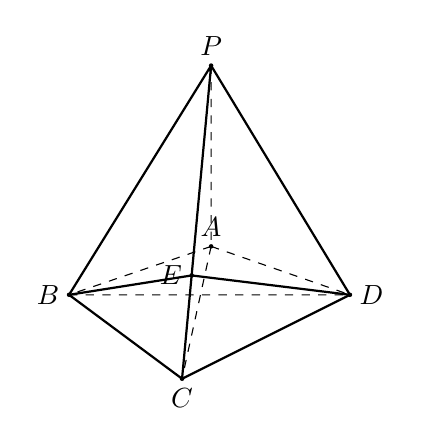
\begin{tikzpicture}[scale=.82,>=stealth]
\coordinate (A) at (0,0);
\coordinate (B) at (-2.2,-.75);
\coordinate (C) at (-.45,-2.05);
\coordinate (D) at (2.15,-.75);
\coordinate (P) at (0,2.8);
\coordinate (E) at (-.3,-.45);

% Visible base edges and lateral edges.
\draw[thick] (B)--(C)--(D);
\draw[thick] (P)--(B) (P)--(C) (P)--(D);
\draw[thick] (E)--(B) (E)--(D);
% Hidden base diagonals/edges and hidden lateral edge.
\draw[dashed] (A)--(B) (A)--(D) (A)--(C) (B)--(D) (P)--(A);
\fill (A) circle (1pt) node[above] {$A$};
\fill (B) circle (1pt) node[left] {$B$};
\fill (C) circle (1pt) node[below] {$C$};
\fill (D) circle (1pt) node[right] {$D$};
\fill (P) circle (1pt) node[above] {$P$};
\fill (E) circle (1pt) node[left] {$E$};
\end{tikzpicture}
\end{center}
\nopagebreak[4]
（1）　证明：$PC\perp$ 平面 $BED$；

（2）　设二面角 $A-PB-C$ 为 $90^\circ$，求 $PD$ 与平面 $PBC$ 所成角的大小。

\end{question}
\begin{question}
\gkti{19}乒乓球比赛规则规定：一局比赛，双方比分在 $10$ 平前，一方连续发球 $2$ 次后，对方再连续发球 $2$ 次，依次轮换。每次发球，胜方得 $1$ 分，负方得 $0$ 分。设在甲、乙的比赛中，每次发球，发球方得 $1$ 分的概率为 $0.6$，各次发球的胜负结果相互独立。甲、乙的一局比赛中，甲先发球。

（1）　求开始第 $4$ 次发球时，甲、乙的比分为 $1$ 比 $2$ 的概率；

（2）　$\xi$ 表示开始第 $4$ 次发球时乙的得分，求 $\xi$ 的期望。

\end{question}
\begin{question}
\gkti{20}设函数 $f(x)=ax+\cos x$，$x\in[0,\pi]$。

（1）　讨论 $f(x)$ 的单调性；

（2）　设 $f(x)\leqslant1+\sin x$，求 $a$ 的取值范围。

\end{question}
\begin{question}
\gkti{21}已知抛物线 $C:y=(x+1)^2$ 与圆 $M:(x-1)^2+\left(y-\dfrac12\right)^2=r^2$（$r>0$）有一个公共点 $A$，且在 $A$ 处两曲线的切线为同一直线 $l$。

（1）　求 $r$；

（2）　设 $m\text{、}n$ 是异于 $l$ 且与 $C$ 及 $M$ 都相切的两条直线，$m\text{、}n$ 的交点为 $D$，求 $D$ 到 $l$ 的距离。

\end{question}
\begin{question}
\gkti{22}函数 $f(x)=x^2-2x-3$，定义数列 $\{x_n\}$ 如下：\linebreak $x_1=2$，$x_{n+1}$ 是过两点 $P(4,5)\text{、}Q_n(x_n,f(x_n))$ 的直线 $PQ_n$ 与 $x$ 轴交点的横坐标。

（1）　证明：$2\leqslant x_n<x_{n+1}<3$；

（2）　求数列 $\{x_n\}$ 的通项公式。

\end{question}